\chapter{平坦座標における地平線と蒸発の熱力学}

\lectureoverview{シュヴァルツシルト計量は地平線において特異になるように見えるが、自由落下する観測者はそこに何ら異常を感じないはずである。この緊張を、地平線近傍の計量を双曲極座標における平坦なミンコフスキー空間へ変換することによって解消する。同じ幾何学が、アリスの落下する記述とボブの加速された外部の記述とを分離する。後半ではエントロピーと温度を展開し、ホーキングの逆質量温度と\(M^3\)の蒸発則を導き、最後に情報の保存が重力の微視的理論に何を要求するかを問う。}

\section{\texorpdfstring{\(r=2GM\)}{r=2GM}における難問}

非常に大きなブラックホールから始めよう。その地平線は曲率が非常に小さいため、そこを落下して通過する観測者は、適度な実験室サイズの領域にわたって、ほとんど空の平坦な時空を見る。壁にぶつかることもなく、通過を告げる局所的な警報も鳴らない。それにもかかわらず、シュヴァルツシルト計量はまさにその半径において何か特異なことが起こると述べているように見える。講義の前半の目的は、これら二つの主張を両立させることである。

我々はmostly-plusの規約を用いる。平坦な時空では、
\begin{equation}
ds^2=-dt^2+dx^2+dy^2+dz^2,
\end{equation}
であるから、時間的worldlineは\(ds^2<0\)を持ち、固有時は\(d\tau^2=-ds^2\)を満たす。これは前の講義で用いた規約の全体的な符号反転である。観測可能な量はその選択に依存しない。

\(c=1\)とすると、シュヴァルツシルト線素は
\begin{equation}
\begin{aligned}
ds^2={}&-\left(1-\frac{2GM}{r}\right)dt^2
+\frac{dr^2}{1-\frac{2GM}{r}}
+r^2d\Omega_2^2,\\
d\Omega_2^2={}&d\theta^2+\sin^2\theta\,d\phi^2 .
\end{aligned}
\label{eq:l03-schwarzschild}
\end{equation}
である。シュヴァルツシルト半径は\(R_s=2GM\)、すなわち\(c\)を復元すれば\(R_s=2GM/c^2\)である。遠方では\(r\gg R_s\)であり、動径方向の両方の係数は平坦空間の値に近づく。しかし\(r=R_s\)では、\(dt^2\)の係数が消え、\(dr^2\)の係数が発散する。それは劇的に見える。問題は、幾何学が劇的なのか、それとも座標だけが劇的なのかである。

\section{二つの座標の教訓}

\subsection{極座標の無害な原点}

通常のユークリッド平面では、
\begin{equation}
ds^2=dx^2+dy^2.
\end{equation}
極座標を導入する。
\begin{equation}
x=\rho\cos\theta,
\qquad
y=\rho\sin\theta .
\end{equation}
微小変位は動径方向の長さ\(d\rho\)と横方向の長さ\(\rho\,d\theta\)を持つから、
\begin{equation}
ds^2=d\rho^2+\rho^2d\theta^2.
\label{eq:l03-polar}
\end{equation}
である。\(\rho=0\)では角度の係数が消える。これは平面の中心を特異にするものではない。そこでは\(\theta\)のどの値も同じ点を指すと述べているだけである。したがって、奇妙な計量の係数は、奇妙な物理ではなく奇妙な座標系を診断しているのかもしれない。

\subsection{双曲極座標}

次にユークリッド平面を\(1+1\)次元ミンコフスキー時空に置き換える。
\begin{equation}
ds^2=-dT^2+dX^2.
\end{equation}
右側のwedge\(X>|T|\)において、
\begin{equation}
X=\rho\cosh\omega,
\qquad
T=\rho\sinh\omega,
\qquad \rho>0 .
\label{eq:l03-rindler-transform}
\end{equation}
と定義する。通常の恒等式\(\cos^2\theta+\sin^2\theta=1\)は
\begin{equation}
\cosh^2\omega-\sinh^2\omega=1.
\end{equation}
に置き換えられる。したがって、\(\rho\)が一定の線は双曲線
\begin{equation}
X^2-T^2=\rho^2.
\end{equation}
である。周期的な角度\(\theta\)とは異なり、rapidity的な座標\(\omega\)は\(-\infty\)から\(+\infty\)まで走る。大きな正の\(\omega\)では、\(\cosh\omega\)と\(\sinh\omega\)はほとんど等しくなり、双曲線は未来のヌル光線\(X=T\)に近づく。

式~\eqref{eq:l03-rindler-transform}を微分すると
\begin{align}
dX&=\cosh\omega\,d\rho+\rho\sinh\omega\,d\omega,\\
dT&=\sinh\omega\,d\rho+\rho\cosh\omega\,d\omega .
\end{align}
が得られる。交差項は相殺され、
\begin{equation}
ds^2=-\rho^2d\omega^2+d\rho^2.
\label{eq:l03-rindler-metric}
\end{equation}
が残る。

\begin{figure}[htbp]
\centering
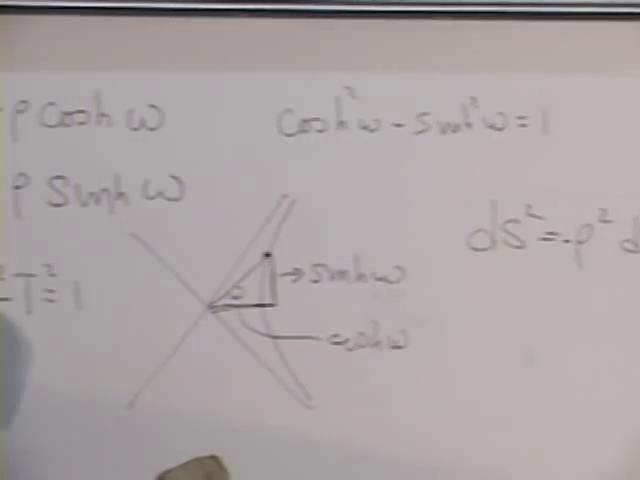
\includegraphics[width=0.72\textwidth]{lecture_03_figure_02.png}
\caption{完成した双曲座標の板書：\(X=\rho\cosh\omega\)、\(T=\rho\sinh\omega\)、単位双曲線の構成、そして\(ds^2=-\rho^2d\omega^2+d\rho^2\)の形の平坦計量。}
\lectureframe{00:16:55.000}
\end{figure}

式~\eqref{eq:l03-rindler-metric}は依然として完全に平坦な時空を記述している。その時間の係数は\(\rho=0\)で消える。ちょうど式~\eqref{eq:l03-polar}の角度の係数が原点で消えるのと同じである。そこでは座標チャートが退化するのであり、時空が退化するのではない。

\section{シュヴァルツシルト地平線へのズームイン}

式~\eqref{eq:l03-schwarzschild}の動径-時間部分に戻る。
\begin{align}
ds^2
&=-\frac{r-2GM}{r}\,dt^2
+\frac{r}{r-2GM}\,dr^2 .
\label{eq:l03-rewritten-schwarzschild}
\end{align}
ここで\(r=2GM\)の狭い近傍だけを調べる。ゆっくり変化する因子では、\(r\)を\(2GM\)で置き換えてよい。因子\(r-2GM\)は保持しなければならない。なぜならそれは地平線で消え、符号を変えるからである。したがって
\begin{equation}
ds^2\approx
-\frac{r-2GM}{2GM}\,dt^2
+\frac{2GM}{r-2GM}\,dr^2 .
\label{eq:l03-near-horizon-r}
\end{equation}

第二項が単に\(d\rho^2\)となるように新しい動径座標\(\rho\)を選ぶ。
\begin{equation}
d\rho^2=\frac{2GM}{r-2GM}\,dr^2.
\end{equation}
地平線の外側で、正の平方根をとり\(r=2GM\)から積分すると
\begin{align}
d\rho&=\sqrt{\frac{2GM}{r-2GM}}\,dr,\\
\rho&=2\sqrt{2GM}\sqrt{r-2GM},\\
\rho^2&=8GM(r-2GM),
\qquad
r-2GM=\frac{\rho^2}{8GM}.
\label{eq:l03-rho-r}
\end{align}
が得られる。式~\eqref{eq:l03-near-horizon-r}に代入すると
\begin{equation}
ds^2\approx
-\frac{\rho^2}{16G^2M^2}\,dt^2+d\rho^2.
\end{equation}
となる。最後にシュヴァルツシルト時間を再スケールし、
\begin{equation}
\omega=\frac{t}{4GM},
\qquad
d\omega^2=\frac{dt^2}{16G^2M^2},
\label{eq:l03-omega}
\end{equation}
を得る。
\begin{equation}
\boxed{ds^2\approx-\rho^2d\omega^2+d\rho^2.}
\label{eq:l03-near-horizon-rindler}
\end{equation}

\begin{figure}[htbp]
\centering
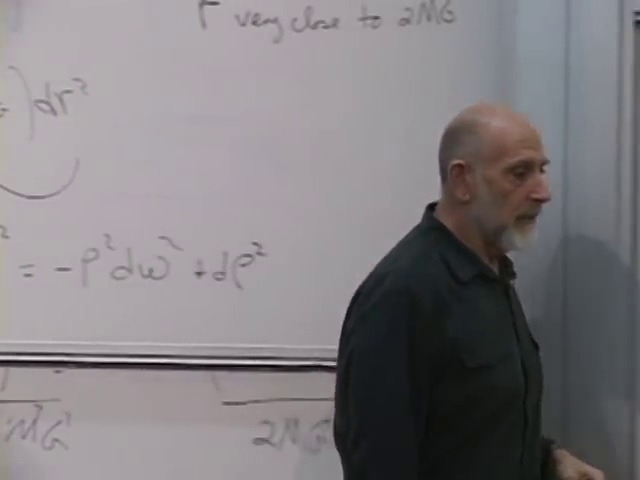
\includegraphics[width=0.70\textwidth]{lecture_03_figure_03.png}
\caption{時間再スケーリング後の板書：地平線近傍のシュヴァルツシルト計量は、平坦なミンコフスキー時空と同じ双曲極座標計量になった。}
\lectureframe{00:31:35.000}
\end{figure}

検査する近傍を地平線に向かって縮めていくと、この近似は際限なく良くなる。それは求められていた局所的な主張を証明している。すなわち、十分に大きな穴に対しては、地平線は異常な座標で書かれた通常の時空である。有限質量のシュヴァルツシルト穴に対して曲率が文字通りゼロであるわけではないが、地平線において有限であり、\(M\) を大きくすることでそこではいくらでも小さくできる。\editorialnote{局所的な曲率スケールは \(R_s^{-2}\) の程度である。リンドラー計量は地平線近傍の局所展開の主要項であり、シュヴァルツシルト幾何全体が大域的に平坦であるという主張ではない。}

\begin{classroomqa}
\audiencequestion{\(r<2GM\) に対して、式~\eqref{eq:l03-rho-r} はこの外部の \(\rho\) を虚数にする。これは物理的な問題を示しているのだろうか。\lecturetimestamp{00:32:30}}
\lecturerresponse{それは同じ座標の破綻を別の形で再現している。現在の座標は外部の楔のために構成されたものであり、地平線を越えて延長するには別の座標が必要である。この特定の \(\rho\) の破綻は、地平線における物理的な事象ではない。}
\end{classroomqa}

\begin{classroomqa}
\audiencequestion{地平線近傍への書き換えにおいて、近似された行は先行する厳密な行からどのように導かれるのか。\lecturetimestamp{00:39:21}}
\lecturerresponse{ゆっくりと変化する \(r\) の出現箇所だけが \(2GM\) に等しいと置かれている。小さな差 \(r-2GM\) はそのまま残されている。それがこの近似であり、\(r\) が \(2GM\) に近づくにつれてますます正確になる。}
\end{classroomqa}

\section{座標の意味}

この変換は次を同定する。
\begin{equation}
\rho=0\quad\Longleftrightarrow\quad r=2GM.
\end{equation}
外部 \(r>2GM\) は右リンドラー楔 \(X>|T|\) である。一定の \(\rho\) の双曲線は、固定されたシュヴァルツシルト半径にとどまる観測者を表す。その楔内のどこかで放出された外向きの光線は、より大きな \(\rho\) のすべての世界線と交差するので、外部の観測者は外向きに通信できる。未来のヌル境界を越えた点は、右の楔へ光信号を送り返すことができない。そのヌル境界が地平線である。

\begin{classroomqa}
\audiencequestion{ここに示された双曲線座標のパッチは、常に地平線の外側の領域を記述するのか。\lecturetimestamp{00:35:22}}
\lecturerresponse{はい。この構成では \(r>2GM\) が \(\rho^2>0\) を与え、事象を右の外部楔に置く。ヌル端 \(\rho=0\) が地平線であり、現在の座標はそれを越えて実の外部座標として続かない。}
\end{classroomqa}

\begin{classroomqa}
\audiencequestion{一定の \(\rho\) の双曲線は、一つの時間を表すのか、それとも一つの距離を表すのか。\lecturetimestamp{00:37:21}}
\lecturerresponse{それは地平線近傍近似において地平線からの一つの固定された固有距離を表し、したがって一つの固定されたシュヴァルツシルト半径を表す。双曲線に沿った運動は、そこに配置された観測者にとっての時間の経過である。}
\end{classroomqa}

固定された \(\rho\) の軌道に沿って、式~\eqref{eq:l03-rindler-metric} は次を与える。
\begin{equation}
d\tau=\rho\,d\omega.
\label{eq:l03-proper-time-rindler}
\end{equation}
したがって \(\omega\) はそれ自体では観測者の固有時ではない。それは双曲線の族に共通の角時間であり、各観測者はそれをその観測者の \(\rho\) で掛ける。ちょうど通常の角度が円の半径で掛けられて弧の長さを与えるのと同じである。

\begin{classroomqa}
\audiencequestion{\(\omega\) は加速する観測者の固有時か。\lecturetimestamp{00:51:45}}
\lecturerresponse{ほとんどそうである。固定された \(\rho\) において、固有時の増分は \(\rho\,d\omega\) である。\(\rho\) の因子が本質的である。}
\end{classroomqa}

\begin{figure}[htbp]
\centering
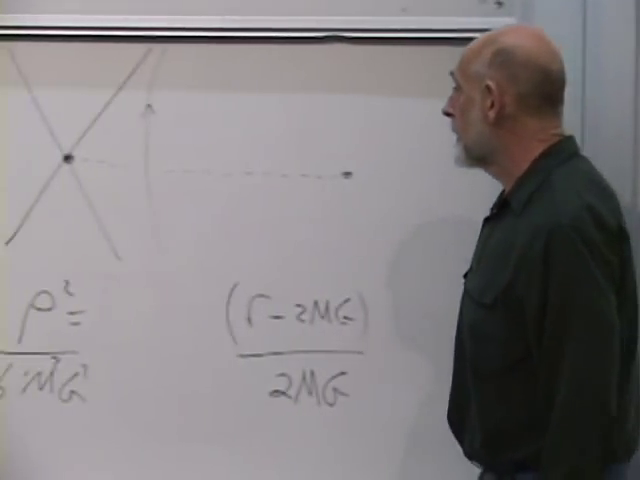
\includegraphics[width=0.72\textwidth]{lecture_03_figure_04.png}
\caption{地平線近傍の因果ボード。交差するヌル境界、外部楔における一定半径の双曲線、そして \(\rho\) と \(r-2GM\) の座標関係。}
\lectureframe{00:34:35.000}
\end{figure}

\begin{figure}[htbp]
\centering
\begin{tikzpicture}[scale=1.04,>=Latex]
  \draw[->] (-0.3,0) -- (4.6,0) node[right] {\(X\)};
  \draw[->] (0,-3.2) -- (0,3.2) node[above] {\(T\)};
  \draw[very thick,blue!55!black] (0,0) -- (3,3);
  \draw[very thick,blue!55!black] (0,0) -- (3,-3);
  \node[blue!55!black,rotate=45] at (0.72,1.02) {future horizon};
  \draw[thick,domain=-1.45:1.45,samples=80] plot ({0.75*cosh(\x)},{0.75*sinh(\x)});
  \draw[thick,domain=-1.25:1.25,samples=80] plot ({1.25*cosh(\x)},{1.25*sinh(\x)});
  \draw[very thick,domain=-1.05:1.05,samples=80] plot ({2.0*cosh(\x)},{2.0*sinh(\x)});
  \node at (3.64,2.18) {Bob: \(\rho=\mathrm{const.}\)};
  \draw[very thick,red!65!black,->] (1.2,-2.9) -- (1.2,2.9);
  \node[red!65!black] at (1.58,-1.75) {Alice};
  \fill[red!65!black] (1.2,1.2) circle (1.7pt);
  \draw[dashed,->] (1.2,0) -- (2.27,1.07);
  \node[align=left] at (3.18,0.80) {\small pre-crossing\\[-0.2em]\small light signal};
\end{tikzpicture}
\caption{ボードの組版された相棒。ボブは加速された一定の \(\rho\) の双曲線に従い、アリスは未来の地平線を通る局所的に慣性の直線に従う。ヌル境界は、アリスにとって局所的な障害となることなく、ボブの因果的アクセスを制限する。}
\end{figure}

\section{アリスは落下し、ボブはホバリングする}

ボブが地平線から固定された距離を保つ一方で、アリスは彼の手を離して落下する。ボブの世界線は双曲線であり、したがって加速されている。アリスの局所的な世界線はほぼ直線である。彼女は有限の固有時間でヌル境界を横切り、局所的な不連続に遭遇しない。

因果的記述は非対称である。アリスが横切った後、彼女からの光はボブに届かないが、ボブが放った光はしばらくの間アリスに届く。ボブは、アリスの有限な落下の次第に早い段階で放たれた信号を受け取る。それらの到達時刻はますます引き離され、周波数は赤方偏移し、強度は弱まる。シュヴァルツシルト時間では、彼は横断そのものを決して見ない。アリスは地平線に漸近的に近づき、それに張り付いて平坦化するように見える。彼女の鼻が平坦化する一方で後頭部が普通のままである、というのではない。あらゆる部分からの信号が同じ極限的な層に圧縮されるのである。

\begin{classroomqa}
\audiencequestion{アリスは横切った後、ボブの光子が彼女に向かって内向きに進むのでボブを見ることができるのか。\lecturetimestamp{00:42:48}}
\lecturerresponse{はい。一方向の因果関係が要点である。ボブの内向きの信号は入ることができるが、アリスの後の外向きの信号はボブへ逃げ戻ることができない。}
\end{classroomqa}

\begin{classroomqa}
\audiencequestion{アリスの足が先に横切り、目が外側に残っているなら、彼女は一時的に自分の足を見失うのか。\lecturetimestamp{00:43:03}}
\lecturerresponse{通常の落下では視覚的な途切れはない。光は足から目まで進むのに常に時間がかかる。関連する信号が到着するころには、彼女の目も横切っている。足が内向きに進み続ける間、頭を外側に保持しようとする激しい試みだけが、異なる破壊的な状況を生むであろう。}
\end{classroomqa}

位置を保持することは非慣性の選択である。ボブにはロケットが必要である。ちょうど床に立っている人には自由落下を避けるために床の上向きの力が必要であるのと同じである。ボブが地平線に近くホバリングするほど、必要な固有加速度は大きくなる。局所リンドラー近似では、その大きさは単位\(c=1\)で\(a=1/\rho\)である。\editorialnote{単位を戻すと、局所リンドラー観測者に対して\(a=c^2/\rho\)となる。厳密に静的シュヴァルツシルト観測者の固有加速度は、地平線に近づくにつれて発散する。}

\begin{classroomqa}
\audiencequestion{講義室に立っているとき、我々は加速しているのか。\lecturetimestamp{00:45:40}}
\lecturerresponse{はい、自由落下系に対してである。床が我々を支えている。床がなければ、あるいはジェットパックがなければ、我々は落下するであろう。}
\end{classroomqa}

\begin{classroomqa}
\audiencequestion{ボブは最終的に、地平線から1プランク長以内にいるアリスを見るのか。そしてその後何が起こるのか。\lecturetimestamp{00:49:24}}
\lecturerresponse{そこでは古典的幾何学的記述が十分でなくなる。プランク長には\(\hbar\)が含まれるので、そこでボブが何を分解できるかを答えるには量子力学が必要である。}
\end{classroomqa}

\begin{classroomqa}
\audiencequestion{一定半径の曲線は、直角のような座標の角で地平線に出会うように見える。そこで微分を取ることができるのか。\lecturetimestamp{00:51:12}}
\lecturerresponse{その点でこの座標チャートに特異なことが起こるが、局所物理には起こらない。他の楔を覆うチャートは人為的な角を取り除く。現在の外部に関する議論では、リンドラー描像が必要な因果的事実をすでに含んでいる。}
\end{classroomqa}

したがって、観測者を指定せずに、アリスが\emph{本当に}横切るのかどうかを問うことは役に立たない。アリスの時計は有限の固有時間で地平線に達する。ボブが受け取る信号列には横断事象が決して含まれない。物理学は、各観測者が何を測定し、それらの記録をどのように比較できるかを問う。

\begin{classroomqa}
\audiencequestion{ボブ自身の観測時間は非有界であるにもかかわらず、ボブはアリスの未来の有限部分しか見ることができない、というのが鋭い主張か。\lecturetimestamp{00:53:33}}
\lecturerresponse{はい。アリスは自分の落下の可視部分に有限の固有時間を割り当てる。理想化された永遠の幾何学では、ボブはますます遅延し赤方偏移したその信号を永遠に受け取るが、地平線横断を超えて彼女が年を取り続けるのを見ることはない。}
\end{classroomqa}

\section{加速地平線だけで十分である}

この因果構造にはブラックホールを必要とするものは何もない。永遠に一様に加速し続けるロケットは、平坦時空内でリンドラー双曲線に沿って進み、信号がそれに追いつけない零境界を持つ。その観測者にとって加速地平線が存在する。慣性観測者は同じ領域を通常のミンコフスキー空間とみなすにもかかわらず、である。

\begin{classroomqa}
\audiencequestion{この現象はブラックホールに固有のものか、それとも任意の地平線で起こるのか。\lecturetimestamp{00:55:25}}
\lecturerresponse{同じ現象は一様に加速する観測者でも起こる。そのような観測者には加速地平線があり、その先の事象を見ることはできない。局所的には、ブラックホールの地平線はその場合と物理的に異ならない。}
\end{classroomqa}

これは等価原理が働いている例である。まず一様加速を理解し、次に重力場の中に同じ局所構造を見出すのである。振り返れば、ブラックホールが受け入れられる以前から、加速の地平線から重力の地平線を予期できたはずである。アインシュタイン自身は、ブラックホールの物理的形成を受け入れなかった。その幾何学が従う理論を与えたにもかかわらず、である。地平線は自由落下する観測者にとっては退屈であり、外にとどまることに固執する観測者にとっては重大な帰結をもつ。これは有効な記述の間の緊張であって、まだパラドックスではない。

\section{熱とエントロピーに戻る}

休憩の後は、熱力学の帽子をかぶろう。前の構成では、ブラックホールは浴槽のように一滴ずつ満たされた。ただし、各滴はおよそ1ビットを運ぶ光子であった。各ビットは地平線の面積をプランク面積程度の量だけ増加させた。正確なエントロピーは
\begin{equation}
S_{\mathrm{BH}}=\frac{k_B A}{4\ell_P^2}.
\end{equation}
講義では、プランクが自分の長さを別様に定義していれば因子\(1/4\)は避けられたはずだと冗談を言う。真剣な点は、次元解析はスケールを固定するが数値係数は固定しないということである。ホーキングの計算がその係数を固定する。\editorialnote{プランク長には標準的な定義\(\ell_P=\sqrt{G\hbar/c^3}\)がある。この慣習と通常の熱力学的エントロピーを固定すれば、因子\(1/4\)は物理的である。これを再定義するという発言は、慣習についての教室での冗談である。}

温度は、指や温度計が直接それを感知するため、初等的に感じられる。エントロピーはしばしばより神秘的に感じられる。この講義はその階層を逆転させる。すなわち、エントロピーとエネルギーを基本的な変数として扱い、温度はエントロピーが変化するときにエネルギーがどれだけ変化しなければならないかから導かれる：
\begin{equation}
dE=T\,dS.
\end{equation}
講義の1ビット単位では\(\Delta S=1\)であるため、ビットを追加または消去する際に伴う最小エネルギーは\(T\)と呼ばれる。注意深さを欠いて---論理的に言えば大ハンマーに相当するもので---消去すると、任意にそれ以上のエネルギーを散逸させうる。この定義は、失われた情報が微視的な環境自由度へ移される際に可能な最小の散逸に関するものである。従来の単位では、1つの二進ビットは\(\Delta S=k_B\ln2\)を担い、可逆的な消去は少なくとも\(k_BT\ln2\)を散逸させる。\editorialnote{これは、講義がエントロピーと温度の両方をエネルギーに基づく自然単位で測ることを選んだために抑制されているランダウアーの規格化である。}

\subsection{1光子の見積もり}

波長がシュヴァルツシルト半径と同程度の光子を選ぶ：
\begin{equation}
\lambda\sim R_s=\frac{2GM}{c^2}.
\end{equation}
そのエネルギーは、\(h\)と\(\hbar\)を区別する\(2\pi\)の慣習を除いて、
\begin{equation}
\Delta E\sim \frac{\hbar c}{\lambda}.
\end{equation}
これが加えられたビットのエネルギーコストなので、
\begin{equation}
k_BT_H\sim\frac{\hbar c}{R_s}
\sim\frac{\hbar c^3}{GM}.
\label{eq:l03-hawking-scale}
\end{equation}
この発見的議論では\(2\)や\(\pi\)のような因子は決定できない。正確なホーキングの結果は
\begin{equation}
\boxed{k_BT_H=\frac{\hbar c^3}{8\pi GM}.}
\label{eq:l03-hawking-exact}
\end{equation}

\begin{figure}[htbp]
\centering
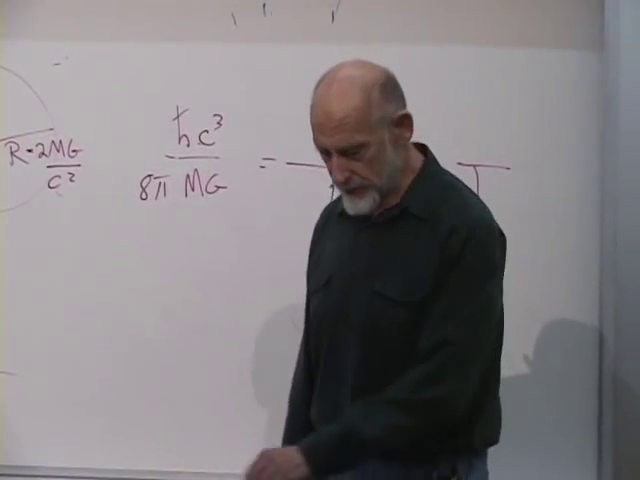
\includegraphics[width=0.72\textwidth]{lecture_03_figure_05.png}
\caption{完成した温度の板書：\(R_s=2GM/c^2\)、1ビットのスケール\(\hbar c/R_s\)、そして正確な\(8\pi\)のホーキング規格化。}
\lectureframe{01:07:48.000}
\end{figure}

ただちに二つの事実が導かれる。第一に、温度は\(\hbar\)とともに消えるので、これは量子効果である。第二に、
\begin{equation}
T_H\propto\frac{1}{M}.
\end{equation}
大きなブラックホールは冷たい。太陽質量1つに対して、
\begin{equation}
T_H\approx6\times10^{-8}\ {\rm K},
\end{equation}
これは講義の\(10^{-8}\,\mathrm{K}\)という見積もりと同じ程度の桁であり、宇宙マイクロ波背景放射の温度約\(2.7\,\mathrm{K}\)よりはるかに低い。

\subsection{負の熱容量}

そのようなブラックホールをより暖かい環境に置く。それはエネルギーを吸収し、質量が増加し、式~\eqref{eq:l03-hawking-exact}によればより冷たくなる。するとさらに吸収しやすくなる。より冷たい環境に置けば逆の暴走が始まる。それは放射し、質量を失い、より熱くなり、より速く放射する。形式的には、
\begin{equation}
C_{\mathrm{BH}}
=\frac{dE}{dT_H}
=c^2\frac{dM}{dT_H}
<0.
\end{equation}

\begin{classroomqa}
\audiencequestion{これが負の比熱という意味ですか。\lecturetimestamp{01:14:08}}
\lecturerresponse{まさにそのとおり。自己重力系はエネルギーを失いながら熱くなりうる。恒星も類似のことをする。放射すると圧力が下がって収縮し、重力圧縮がその温度を上げる。}
\end{classroomqa}

孤立したブラックホールがそれゆえ非物理的になるわけではない。今日の宇宙では、恒星質量のブラックホールは周囲より冷たく、主に吸収する。宇宙が膨張し背景が冷えるにつれ、バランスはやがて逆転し、蒸発が支配的になりうる。実効的に無限の熱浴との単純な平衡は不安定である。\editorialnote{境界条件が重要である。ブラックホールは有限の反射空洞の中や、適切な大きなブラックホールに対しては反ド・ジッター時空の中で安定化されうる。ここで述べた不安定性は、漸近的に平坦な通常の熱浴の場合である。}

\section{蒸発則}

スケーリングの導出にあたっては、参考書がない状況を想像し、記憶している方程式が最も短くなる単位を選ぶ：
\begin{equation}
c=\hbar=G=k_B=1.
\end{equation}
これらはプランク単位である。講義で引用された特徴的なスケールは
\begin{equation}
\ell_P\sim10^{-35}\ {\rm m},
\qquad
t_P\sim10^{-43}\ {\rm s},
\qquad
m_P\sim10^{-8}\ {\rm kg}.
\end{equation}
プランク質量はおおよそ目に見える塵の粒ほどであるが、プランク長とプランク時間は極めて小さい。\(c=1\) であるから、\(t_P\) は単に \(\ell_P\) を光が横切る時間である。

穴を黒体として扱う。すなわち、完全に暗いままでなければならない物体ではなく、熱的な放射体とみなす。それは電磁放射を放出でき、原理的にはグラビトンを含む他の利用可能な種も放出しうる。放射は表面を通って出ていくので、放射されるパワーは放射面積に比例する。シュテファン--ボルツマンのスケーリングは
\begin{equation}
L=-\frac{dE}{dt}\sim A T^4.
\end{equation}
プランク単位では \(E=M\)、\(R_s\sim M\)、\(A\sim R_s^2\sim M^2\)、\(T\sim R_s^{-1}\sim M^{-1}\) である。したがって
\begin{align}
-\frac{dM}{dt}
&\sim R_s^2\left(\frac{1}{R_s}\right)^4
\sim\frac{1}{R_s^2}
\sim\frac{1}{M^2},\\
-M^2\frac{dM}{dt}&\sim1,\\
-\frac{d(M^3)}{dt}&\sim1.
\label{eq:l03-evap-scaling}
\end{align}
1次の係数を無視すると、寿命は
\begin{equation}
\boxed{t_{\mathrm{evap}}\sim M^3.}
\label{eq:l03-lifetime}
\end{equation}

\begin{figure}[htbp]
\centering
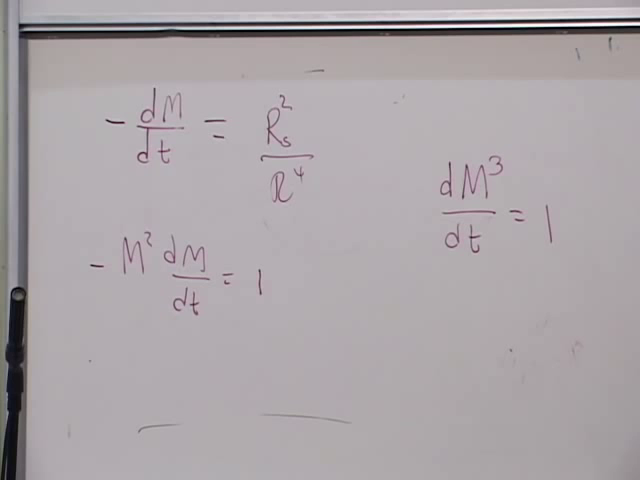
\includegraphics[width=0.72\textwidth]{lecture_03_figure_06.png}
\caption{妨げのない蒸発盤：光度は\(-dM/dt\sim1/M^2\)を与え、したがって\(M^3\)の一様な減少と、初期質量の三乗に比例する寿命が得られる。}
\lectureframe{01:23:20.000}
\end{figure}

この模式的なシュテファン--ボルツマン的取り扱いは、グレイボディ因子と粒子種の数を抑圧している。中性で回転しない穴について、最も単純な無質量放出近似で定数を復元すると
\begin{equation}
t_{\mathrm{evap}}
=\frac{5120\pi G^2M_0^3}{\hbar c^4}.
\label{eq:l03-exact-lifetime}
\end{equation}
この係数は編集上の補完であり、講義は頑健な \(M_0^3\) 依存性のみを導出している。

\subsection{太陽、山、キログラムのスケール}

太陽の質量は\(M_\odot\sim10^{30}\,\mathrm{kg}\sim10^{38}m_P\)である。これを三乗し、一プランク時間を掛けると、講義の意図的に粗い連鎖
\begin{equation}
t_{\mathrm{evap}}\sim10^{114}t_P
\sim10^{71}\ {\rm s}
\sim10^{64}\ {\rm yr}.
\end{equation}
が得られる。どちらの推定値も、宇宙のおよそ\(10^{10}\)年の年齢より途方もなく長い。式~\eqref{eq:l03-exact-lifetime}の係数を復元すると、標準的な太陽質量の推定値は約\(2\times10^{67}\)年になる。\editorialnote{この違いは予想されるものである。黒板での計算はすべての数値定数を落とし、プランクスケールを十の冪で丸めている。その目的は質量の三乗スケーリングであり、精密な寿命天文学ではない。}

次にクラスは\emph{山の質量}の穴を試す。教室での粗い値\(M\sim10^{10}\,\mathrm{kg}\)、したがって\(M\sim10^{18}m_P\)に落ち着き、
\begin{equation}
t_{\mathrm{evap}}\sim10^{54}t_P
\sim10^{11}\ {\rm s}
\sim10^4\ {\rm yr}.
\end{equation}
を得る。これは黒板で実際に行われた算術を保持している。その質量を動機づけるために用いられた言葉による幾何学---およそ\(100\,\mathrm{km}^3\)の岩石---は、実際にははるかに重く、正確な寿命の係数も結果を大きく変えるであろう。\editorialnote{通常の岩石密度では、\(100\,\mathrm{km}^3\)は\(10^{14}\,\mathrm{kg}\)の程度であり、\(10^{10}\,\mathrm{kg}\)ではない。\(10^{10}\,\mathrm{kg}\)に対して、式~\eqref{eq:l03-exact-lifetime}は\(10^6\)年の程度の寿命を与える。これらの補正は、寿命が質量の三乗として減少するという講義の教訓を変えない。}

\begin{classroomqa}
\audiencequestion{質量がわずか一キログラムのブラックホールは極端に小さいだろうか？\lecturetimestamp{01:29:14}}
\lecturerresponse{はい。半径は質量に比例し、太陽質量は数キロメートルに対応するので、一キログラムのシュヴァルツシルト半径は約\(10^{-27}\,\mathrm{m}\)である。そのような穴はまた極端に高温で短命であろう。}
\end{classroomqa}

\begin{classroomqa}
\audiencequestion{これらの蒸発の推定は周囲温度がゼロであると仮定しているのか？\lecturetimestamp{01:29:53}}
\lecturerresponse{それらは周囲が穴より冷たく、正味のエネルギーが外へ流れる場合に適用される。より高温の環境は代わりにブラックホールにエネルギーを供給する。ホーキング温度が現在の背景放射と一致する質量は演習問題として残されている。}
\end{classroomqa}

目安として、\(T_H=2.7\,\mathrm{K}\) と置くと \(M\) は \(10^{22}\,\mathrm{kg}\) の程度となり、シュヴァルツシルト半径は \(10^{-4}\,\mathrm{m}\) の程度となる。\editorialnote{これは講義で出された演習問題を評価するものであり、話された導出の一部ではない。}

\section{計量の下には何がなければならないか？}

\begin{classroomqa}
\audiencequestion{どのような機構が光子をブラックホールから出させるのか？\lecturetimestamp{01:30:53}}
\lecturerresponse{放射の微視的機構を与える前に、エントロピーの原因となる自由度を同定しなければならない。熱力学的議論は、それらの変数をまだ明示的に示すことなく、何が存在しなければならないかを制約する。}
\end{classroomqa}

類推は流体力学である。流体力学は、すべての分子を追跡することなく、滑らかな密度場と速度場を記述する。それにもかかわらず、エントロピーは、同じ滑らかな状態の背後に多くの隠れた微視的配置があることを明らかにする。同様に、古典的一般相対論は滑らかな計量を記述するが、ブラックホールエントロピーによって数えられる多数の微視的自由度を露わにしない。面積則とホーキング放射は、アインシュタインの理論が有効な巨視的記述であることの手がかりである。

\begin{classroomqa}
\audiencequestion{ブラックホールがエネルギーを放射するなら、それは情報を放射すると言うのと同じことで、成長中に飲み込まれた情報が蒸発中に戻ってくるのだろうか？\lecturetimestamp{01:33:27}}
\lecturerresponse{それが要請である。完全な時間発展が情報を保存するなら、出ていく放射は最終的に、ブラックホールを形成した可能な状態を区別できなければならない。これは依然として、物質が事象の地平面を横切るという因果的な描像と折り合いをつけなければならない。}
\end{classroomqa}

エネルギーの流れだけでは情報を指定するのに十分ではない。完全に熱的な密度行列は、詳細な初期状態を忘れつつエネルギーを運ぶことができる。ユニタリーな記述では、必要な情報は放出された量子間の微細な相関に符号化されている。\editorialnote{この区別は情報問題の現代的な形を明示する。それは講義で提起された問いを鋭くするのであって、変えるのではない。}

\section{情報保存の構造的原理としての位置づけ}

\begin{classroomqa}
\audiencequestion{情報の保存は本当に基本原理なのだろうか？\lecturetimestamp{01:34:13}}
\lecturerresponse{それは最も基本原理的なものの一つである。異なる初期状態がまったく同じ最終状態へと発展しうるなら、法則は自らの過去を消去してしまうことになる。通常の保存則は対称性だけでなく、可逆なハミルトニアン、すなわちユニタリーな形の時間発展にも依拠している。}
\end{classroomqa}

講義がそうするように、滑っている消しゴムをすべて単に静止させる架空の基本法則を想像してみよ。異なる初速度がすべて同じ状態に終わる。最終状態の消しゴムはもはやその履歴を区別しない。情報は破壊されている。運動量と力学的エネルギーも消える。現実の摩擦は微視的レベルではこうはならない。運動量とエネルギーは机、空気、熱的自由度へと移る。

完全に一様な無限の卓上であっても並進対称性をもつが、それでも架空の減衰法則は消しゴムを停止させうる。したがって並進対称性だけでは、そのような非ハミルトニアン的規則から運動量保存を導くのに十分ではない。ネーターの定理は作用原理とそれに伴う可逆な力学を前提とする。ここで用いられている言葉では、対称性と情報保存的な力学が保存則を与える。

\begin{classroomqa}
\audiencequestion{情報保存は因果性よりも基本原理なのだろうか？\lecturetimestamp{01:37:00}}
\lecturerresponse{それらは同程度に基礎的なレベルにある異なる原理である。因果性はまず正確に述べられなければならない---たとえば、信号は許された因果構造の外へ逆向きに伝播できないということ---が、どちらの原理も単純に他方を置き換えることはできない。}
\end{classroomqa}

\begin{classroomqa}
\audiencequestion{ハミルトン力学で議論される位相空間の面積保存は、この考えの古典版なのだろうか？\lecturetimestamp{01:37:38}}
\lecturerresponse{そのとおりである。リウヴィルの定理は、ハミルトン流が位相空間の体積を保存すると述べている。可能な初期状態の雲は、より小さな体積へと崩壊して区別を消去することはできない。量子力学では対応する主張はユニタリー性である。内積、したがって直交状態間の区別が保存される。}
\end{classroomqa}

古典的には、
\begin{equation}
\frac{d}{dt}\,\mathrm{Vol}_{\Gamma}=0,
\end{equation}
ハミルトン流によって輸送される位相空間領域に対して成り立つ。量子力学的には、
\begin{equation}
\begin{aligned}
\ket{\psi(t)}&=U(t)\ket{\psi(0)},\\
U^\dagger U&=I,\\
\braket{\psi(t)}{\phi(t)}
&=\braket{\psi(0)}{\phi(0)}.
\end{aligned}
\end{equation}
これらは、微視的な区別が時間発展を通じて生き残るという主張の正確な形である。

\section{エントロピーはどちらに依存するのか？}

最後のやり取りは情報理論的エントロピーに戻る。微視的な選択肢に対する確率\(p_i\)が与えられたとき、
\begin{equation}
S=-k_B\sum_i p_i\ln p_i
\label{eq:l03-shannon}
\end{equation}
熱力学的単位では、あるいは\(k_B\)を付けずに無次元のシャノンエントロピーとして表される。

\begin{figure}[htbp]
\centering
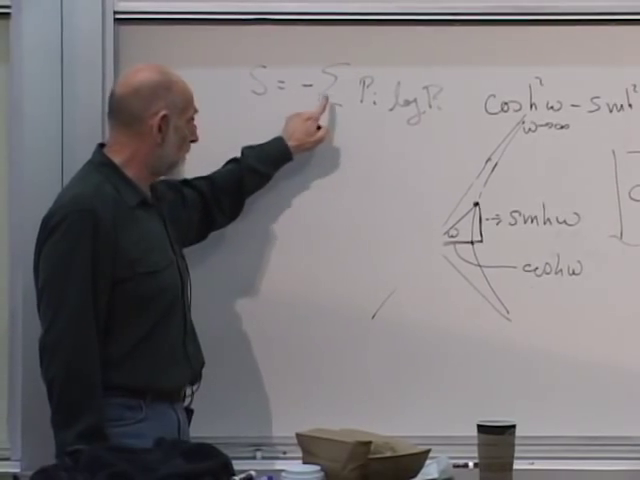
\includegraphics[width=0.72\textwidth]{lecture_03_figure_07.png}
\caption{最後の板書の式\(S=-\sum_i p_i\log p_i\)は、確率分布とそれから計算される単一のエントロピー値を区別しながら書かれたものである。}
\lectureframe{01:40:32.000}
\end{figure}

\begin{classroomqa}
\audiencequestion{エントロピーを最大化することが確率分布を定義するのであって、確率がエントロピーを定義するのではないのか？\lecturetimestamp{01:38:33}}
\lecturerresponse{確率分布は式~\eqref{eq:l03-shannon}を通じて一つのエントロピー値を定める。一つの数からすべての\(p_i\)を再構成することはできない。エントロピーの最大化が分布を選び出せるのは、規格化や、固定された平均エネルギーなどの他の制約も与えられた後だけである。}
\end{classroomqa}

この区別が講義をまさに正しい最前線で終わらせる。滑らかな幾何学は地平面へと導いた。地平面は熱力学へと導いた。熱力学は隠れた自由度を露わにした。そして情報保存は今や、それらの自由度が、ブラックホールに入った区別を消去することなく発展することを要求している。その機構はまだ与えられていない。代わりに幾何学と帳簿付けが、成功するどんな微視的理論も説明しなければならないことを明らかにしたのである。
